%%%%%%%%%%%%%%%%%%%%%%%%%%%%%%%%%%%%%%%%%
% Document Author: Plinio H. Vargas
% Course: CS-532, Spring 2016 at Old Dominion University
%
% Structured General Purpose Assignment
% LaTeX Template
%
% This template has been downloaded from:
% http://www.latextemplates.com
%
% Original template author:
% Ted Pavlic (http://www.tedpavlic.com)
%
% Note:
% The \lipsum[#] commands throughout this template generate dummy text
% to fill the template out. These commands should all be removed when 
% writing assignment content.
%
%%%%%%%%%%%%%%%%%%%%%%%%%%%%%%%%%%%%%%%%%
%----------------------------------------------------------------------------------------
%	PACKAGES AND OTHER DOCUMENT CONFIGURATIONS
%----------------------------------------------------------------------------------------

\documentclass{article}

\usepackage{fancyhdr} % Required for custom headers
\usepackage{lastpage} % Required to determine the last page for the footer
\usepackage{extramarks} % Required for headers and footers
\usepackage{listings}
\usepackage{graphicx} % Required to insert images
\usepackage{lipsum} % Used for inserting dummy 'Lorem ipsum' text into the template
\usepackage[bookmarks,bookmarksopen,bookmarksdepth=2]{hyperref} % for bookmarks
\usepackage{enumerate}
\usepackage{csquotes} % for quoting things
\usepackage{multirow}
\usepackage{amsmath}
\usepackage{caption}
\usepackage{navigator}%\usepackage{caption}
\usepackage[shortlabels]{enumitem}
\usepackage{enumitem}
\usepackage{lmodern}
\usepackage[utf8]{inputenc}
%\usepackage[table]{xcolor}% http://ctan.org/pkg/xcolo
\usepackage[dvipsnames]{xcolor}
\usepackage{longtable}
\usepackage{textcomp}
\usepackage{url}
\usepackage{import}
\usepackage{float}
\usepackage{dashrule} % for dashline
\usepackage{keystroke}
\usepackage{amssymb}

\lstdefinestyle{numbers}
{ frame=tb,
  language=python,
  aboveskip=3mm,
  belowskip=3mm,
  showstringspaces=false,
  columns=flexible,
  basicstyle={\small\ttfamily},
  numbers=left,
  numberstyle=\tiny\color{gray},
  keywordstyle=\color{blue},
  commentstyle=\color{OliveGreen},
  stringstyle=\color{purple},
  breaklines=true,
  breakatwhitespace=true,
  tabsize=3
}

\lstdefinestyle{nonumbers}
{ frame=shadowbox,
  language=python,
  aboveskip=3mm,
  belowskip=3mm,
  showstringspaces=false,
  columns=flexible,
  basicstyle={\small\ttfamily},
  numbers=none,
  numberstyle=\tiny\color{gray},
  keywordstyle=\color{blue},
  commentstyle=\color{OliveGreen},
  stringstyle=\color{purple},
  breaklines=true,
  breakatwhitespace=true,
  tabsize=3
}

\lstdefinestyle{mybox}
{
	basicstyle={\small\ttfamily},
    numbers=left,
    numberstyle=\tiny\color{gray},
    stepnumber=1,
    numbersep=5pt,
    showspaces=false, % don't show spaces by adding underscores
    showstringspaces=false, % don't underline spaces in strings
    showtabs=false, % don't show tabs with underscores
    frame=shadowbox,
    tabsize=4,
    captionpos=b,
    breaklines=true,
    breakatwhitespace=false,
  	keywordstyle=\color{blue},
	commentstyle=\color{OliveGreen},
  	stringstyle=\color{purple},    
    rulesepcolor=\color{red!20!green!20!blue!20},
    numberbychapter=false,
    stringstyle=\color{purple},
}


\providecommand{\providehyphenmins}[2]{}

% Margins
\topmargin=-0.45in
\evensidemargin=0in
\oddsidemargin=0in
\textwidth=6.5in
\textheight=9.0in
\headsep=0.25in 

\linespread{1.1} % Line spacing
\newcommand*{\medtau}{\mathbin{\scalebox{1.5}{$\tau$}}}% increase size of tau
\newcommand*{\medtaub}{\mathbin{\scalebox{1.5}{$\tau_b$}}}% increase size of tau_b
\newcommand\multibrace[3]{\rdelim\}{#1}{3mm}[\pbox{#2}{#3}]}

% Set up the header and footer
\pagestyle{fancy}
\lhead{\hmwkAuthorName} % Top left header
\chead{\hmwkShortClass\ (\hmwkClassInstructor\ \hmwkClassTime): \hmwkShortTitle} % Top center header
%\rhead{\firstxmark} % Top right header
\rhead{} % Top right header
\lfoot{\lastxmark} % Bottom left footer
\cfoot{} % Bottom center footer
\rfoot{Page\ \thepage\ of\ \pageref{LastPage}} % Bottom right footer
\renewcommand\headrulewidth{0.4pt} % Size of the header rule
\renewcommand\footrulewidth{0.4pt} % Size of the footer rule

\setlength\parindent{0pt} % Removes all indentation from paragraphs

%----------------------------------------------------------------------------------------
%	DOCUMENT STRUCTURE COMMANDS
%	Skip this unless you know what you're doing
%----------------------------------------------------------------------------------------

% Header and footer for when a page split occurs within a problem environment
\newcommand{\enterProblemHeader}[1]{
\nobreak\extramarks{#1}{#1 continued on next page\ldots}\nobreak
\nobreak\extramarks{#1 (continued)}{#1 continued on next page\ldots}\nobreak
}

% Header and footer for when a page split occurs between problem environments
\newcommand{\exitProblemHeader}[1]{
\nobreak\extramarks{#1 (continued)}{#1 continued on next page\ldots}\nobreak
\nobreak\extramarks{#1}{}\nobreak
}

\newcounter{sub}[section]
\newenvironment{sub}[1][]{\stepcounter{sub}\thesub #1}{ }

\setcounter{secnumdepth}{0} % Removes default section numbers
\newcounter{homeworkProblemCounter} % Creates a counter to keep track of the number of problems
\newcommand{\sectionNumber}{\arabic{homeworkProblemCounter}.\sub }


\newcommand{\homeworkProblemName}{}
\newenvironment{homeworkProblem}[1][Problem \arabic{homeworkProblemCounter}]{ % Makes a new environment called homeworkProblem which takes 1 argument (custom name) but the default is "Problem #"
\stepcounter{homeworkProblemCounter} % Increase counter for number of problems
\setcounter{sub}{0}
\renewcommand{\homeworkProblemName}{#1} % Assign \homeworkProblemName the name of the problem
\
\section{\homeworkProblemName} % Make a section in the document with the custom problem count
\enterProblemHeader{\homeworkProblemName} % Header and footer within the environment
}{
\exitProblemHeader{\homeworkProblemName} % Header and footer after the environment
}

\newcommand{\problemAnswer}[1]{ % Defines the problem answer command with the content as the only argument
\noindent\framebox[\columnwidth][c]{\begin{minipage}{0.98\columnwidth}#1\end{minipage}} % Makes the box around the problem answer and puts the content inside
}

\newcommand{\homeworkSectionName}{}
\newenvironment{homeworkSection}[1]{ % New environment for sections within homework problems, takes 1 argument - the name of the section
\renewcommand{\homeworkSectionName}{#1} % Assign \homeworkSectionName to the name of the section from the environment argument
\subsection{\homeworkSectionName} % Make a subsection with the custom name of the subsection
\enterProblemHeader{\homeworkProblemName\ [\homeworkSectionName]} % Header and footer within the environment
}{
\enterProblemHeader{\homeworkProblemName} % Header and footer after the environment
}
   
%----------------------------------------------------------------------------------------
%	NAME AND CLASS SECTION
%----------------------------------------------------------------------------------------

\newcommand{\hmwkTitle}{\\Assignment\ \#6: \\Data Visualization} % Assignment title
\newcommand{\hmwkShortTitle}{Assignment 6} % Assignment title
\newcommand{\hmwkDueDate}{Thursday,\ March 17,\ 2016} % Due date
\newcommand{\hmwkClass}{CS-432/532 Introduction to Web Science} % Course/class
\newcommand{\hmwkShortClass}{CS-432/532 Web Science} % Course/class
\newcommand{\hmwkClassTime}{- Spring 2016} % Class/lecture time
\newcommand{\hmwkClassInstructor}{Dr.  Michael L. Nelson} % Teacher/lecturer
\newcommand{\hmwkAuthorName}{Plinio Vargas} % Your name
\newcommand{\hmwkAuthorEmail}{pvargas@cs.odu.edu} % Your name
%------------------------------------------------------------
% Algorithm declaration
%------------------------------------------------------------
\lstnewenvironment{algorithm}[1][] %defines the algorithm listing environment
{   
    %\refstepcounter{nalg} %increments algorithm number
    \captionsetup{labelsep=colon} %defines the caption setup for: it ises label format as the declared caption label above and makes label and caption text to be separated by a ':'
    \lstset{ %this is the stype
        frame=tB,
        numbers=left, 
        mathescape=true,
        numberstyle=\tiny,
        basicstyle={\small\ttfamily}, 
        keywordstyle=\color{blue}\bfseries\em,
        keywords={,input, output, return, 
                   datatype, function, in, 
                   if, else, for, foreach, 
                   while, write, begin, end, 
        } %add the keywords you want, or load a language as Rubens explains in his comment above.
        numbers=left,
        xleftmargin=.04\textwidth,
        #1 % this is to add specific settings to an usage of this environment (for instnce, the caption and referable label)
    }
}
{}
%----------------------------------------------------------------------------------------
%	TITLE PAGE
%----------------------------------------------------------------------------------------

\title{
\vspace{2in}
\textmd{\textbf{\hmwkClass:\ \hmwkTitle}}\\
\normalsize\vspace{0.1in}\small{Due\ on\ \hmwkDueDate}\\
\vspace{0.1in}\large{\textit{\hmwkClassInstructor\ }}
\vspace{3in}
}

\author{\textbf{\hmwkAuthorName} \\ \hmwkAuthorEmail}
\date{} % Insert date here if you want it to appear below your name

%----------------------------------------------------------------------------------------
%	EMBEDDED FILE
%----------------------------------------------------------------------------------------
%\embeddedfile{KarateClub}{../KarateClub.py}
%\embeddedfile{DrawOriginalClub}{../DrawOriginalClub.py}
%----------------------------------------------------------------------------------------
%	START OF DOCUMENT
%----------------------------------------------------------------------------------------
\begin{document}

\clearpage\maketitle
\thispagestyle{empty}

%----------------------------------------------------------------------------------------
%	TABLE OF CONTENTS
%----------------------------------------------------------------------------------------

%\setcounter{tocdepth}{1} % Uncomment this line if you don't want subsections listed in the ToC

\newpage
\clearpage\tableofcontents
\listoffigures
\lstlistoflistings
\listoftables

\thispagestyle{empty}
\newpage
\setcounter{page}{1}

%----------------------------------------------------------------------------------------
%	Problem 1
%----------------------------------------------------------------------------------------
\begin{homeworkProblem}% Custom section title
\vspace*{10pt} % Question
D3 graphing (5 points) \\

Use D3 to visualize your Twitter followers.  Use my twitter account ("@phonedude\_mln") if you do not have $>=$ 50 followers.  For example, @hvdsomp follows me, as does @mart1nkle1n.  They also follow each other, so they would both have links to me and links to each other.\\

To see if two users follow each other, see: \url{https://dev.twitter.com/rest/reference/get/friendships/show}\\

Attractiveness of the graph counts!  Nodes should be labeled (avatar images are even better), and edge types (follows, following) should be marked.\\

Note: for getting GitHub to serve HTML (and other media types), see: \url{http://stackoverflow.com/questions/6551446/can-i-run-html-files-directly-from-github-instead-of-just-viewing-their-source}\\

Be sure to include the URI(s) for your D3 graph in your report. \\

\subsection{1.1 Approach}
The twitter account for \textbf{Jose Antonio Olvera}, whom follows Dr. Nelson, was used as our data-set \textbf{\textit{S}} for problem 1. This problem was divided into two sub-problems: extracting the data and plotting the graph.

\subsubsection{1.1.1 Extracting the data}
Listing \ref{lst:twitterapi}  is a python program implemented to extract the data. It accomplishes the following:
\begin{enumerate}[a.]
	\item Obtains $S$'s followers Twitter's ID account using tweepy API \cite{tweepy}. Lines 10-16
	\item All IDs, including $S$, are placed into an array \textbf{\textit{A}}. Lines 20-21.
	\item Iterates through all elements in $A$, extracting its followers and other important information, such as name, screen name, number of friends, etc. Followers of each element are placed into an array \textbf{\textit{B}}. Lines 28-56
	\item Only $B$'s friends in $A$ are needed, then $B = A \cup B$. Lines 36-39. 
	\item The collection of all $B$s arrays are saved into a JSON file. Lines 59-61.
\end{enumerate}

\lstinputlisting[language=Python,
                 style=mybox, 
                 captionpos=t,
                 caption={TwitterAPI.py},
                 label={lst:twitterapi},
				 linerange={10-74},
				 firstnumber=10                 
                 ]
{../../lib/TwitterAPI.py}
\newpage
At the time our data-set has retrieved its size was of 53 elements. There is a request number limitations of 15,  to extract Twitter's user information.  Lines 50-52 catches that error and wait for 15 minutes to continue with the information extraction.\\

Some Twitter users may have privacy settings in their accounts, so their information cannot be retrieved through the API. See section Excluded Data. Lines 68-74.

\subsubsection{1.1.2 Plotting the Graph}
Although we have the data from 1.1.1 to plot the graph, it does not have detail information on how nodes link. $<ReshapeData.py>$ accomplishes the job. It creates within a file two JSON dictionaries: \textbf{nodes}, containing all elements characteristics and \textbf{links}, a source pointing to a target. It also adds a new characteristic to the node: color. It determines how close is the friendship between any node with \textbf{\textit{A}}. 


\begin{figure}[!h]
\center
\caption{Color Scheme} \label{fig:1}
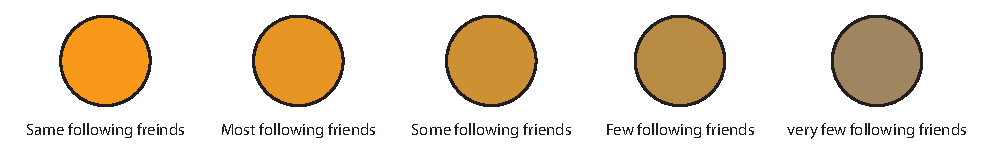
\includegraphics[scale=.85]{images/graph-color.pdf}
\caption*{\scriptsize Figure \ref{fig:1} represents a color scheme showing how similar is any particular node with data-set $A$ in relation to its followers.}
\end{figure}

\lstinputlisting[language=Python,
                 style=mybox, 
                 captionpos=t,
                 caption={ReshapeData.py},
                 label={lst:reshape},
				 linerange={46-81},
				 firstnumber=46                 
                 ]
{../ReshapeData.py}

\vspace*{5mm}
In order to make the graph appealing in terms of friendship colors some test were conducted to capture different similarity levels. As a result, if any particular node has:

\begin{enumerate}[a. ]
	\item If $>$ 20\% of $N$ followers are are also following $A$, then $N$ is color coded as having similar followers as $A$.
	\item If node $N$ has $>$ 14\% and $<$ 20\% of $A$ followers then $N$ is color coded as having most of its followers following $A$.
	\item If node $N$ has $>$ 10\% and $<$ 14\% of $A$ followers then $N$ is color coded as having some its followers are following $A$.	
	\item If node $N$'s has $>$ 4\% and $<$ 14\% of $A$ followers then $N$ is color coded as having few followers following $A$.
		\item If node $N$'s has $<$ 4\% of $A$ followers then $N$ is color coded as very few of $N$'s followers are following $A$.
\end{enumerate}

The color code scheme is implemented in lines 49-62 of $<ReshapeData.py>$. The rest of the code just dump the data into \textbf{\textit{jose.json}}, which is the input file for our Data-Driven Document. \textbf{The color code scheme is not accurate in a English grammar context, but it gives a quick view how closer are their followers network}\\

\textbf{Data Visualization:}\\
Various features from different D3JS sites were used to enhance graph appearance.\\

\begin{tabular}{l l}
	Zooming and dragging & \url{http://bl.ocks.org/mbostock/6123708} \cite{zooming}\\
    Mouseover Tip-tool &  \url{ http://bl.ocks.org/Caged/6476579} \cite{tip-tool}\\
	Directed graph & \url{http://bl.ocks.org/mbostock/1153292}\cite{directed}\\
	Mouseover link hightlight & \url{http://p.migdal.pl/wizualizacja-wolnych-lektur/polish_books_themes.html} \cite{polish-books}\\
	D3 Markers & \url{http://bl.ocks.org/dustinlarimer/5888271}	\cite{d3-markers}
\end{tabular} 

\newpage
\subsection{1.2 Excluded Data}
\vspace*{50mm}
%----------------------------------------------------------------------------------------
%	Table1
%----------------------------------------------------------------------------------------
\import{./}{table-1.tex}

\newpage
\subsection{1.3 Solution}
\begin{figure}[!h]
\center
\caption{Jose A. Olvera Followers Network Graph} \label{fig:graph}
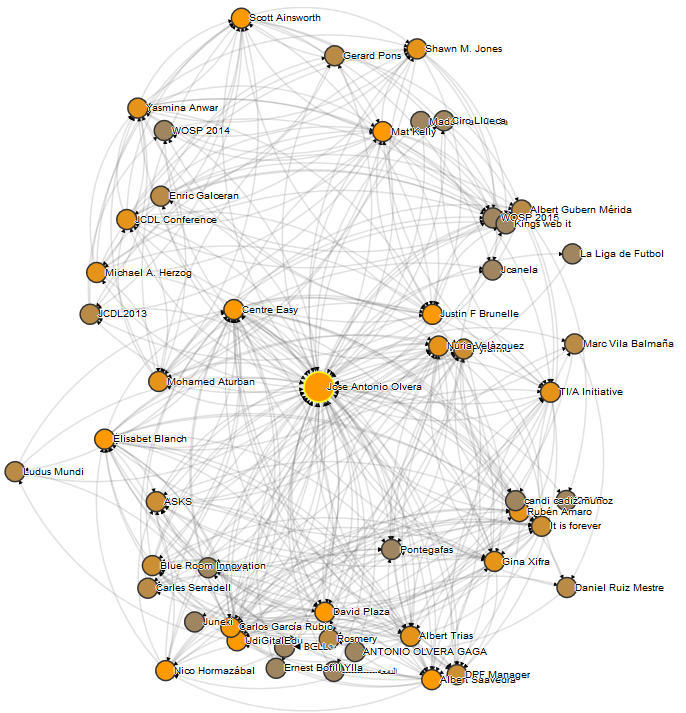
\includegraphics[scale=.85]{images/directed-graph.png}
\caption*{\scriptsize Figure \ref{fig:graph} represents a color scheme showing how similar are the followers of any particular node with $A$ followers. Node $A$ (Jose Antonio Olvera) has a larger radius and a yellow stripe around to distinguish it from the rest of the nodes in the graph.}
\end{figure}

\end{homeworkProblem}

%----------------------------------------------------------------------------------------
%	Problem 2 Extra Credit 1 Point
%----------------------------------------------------------------------------------------
\newpage
\begin{homeworkProblem}
Gender homophily in your Twitter graph (5 points)\\

Take the Twitter graph you generated in question \#1 and test for male-female homophily.  For the purposes of this question you can consider the graph as undirected (i.e., no distinction between "follows" and "following").  Use the twitter name (not "screen name"; for example "Michael L. Nelson" and not \enquote{@phonedud\_mln}) and programatically determine if the user is male or female.  Some sites that might be useful:\\

\url{https://genderize.io/}\\
\url{https://pypi.python.org/pypi/gender-detector/0.0.4}\\

Create a table of Twitter users and their likely gender.  List any accounts that can't be determined and remove them from the graph.\\

Perform the homophily test as described in slides 11-15, Week 7.\\

Does your Twitter graph exhibit gender homophily?\\

\subsection{2.1 Approach}
We we used the same data generated in problem 1 to solve this problem. However, we filtered the data set by injecting the first name of each node with gender\_detector python library. The iteration is shown in the listing below:

\lstinputlisting[language=Python,
                 style=mybox, 
                 captionpos=t,
                 caption={GetGender.py},
                 label={lst:getgender},
				 linerange={20-35},
				 firstnumber=20                 
                 ]
{../GetGender.py}

\vspace{5mm}
The result file can be seen on Table \ref{tab:likely-gender}. To complete our graph and generate a solution we use the same approach as in 1.1.2, but we added an extra field to the nodes: gender, and we placed all linking edges into a set, thus eliminating the extra edge between two nodes having a bi-directional relationship. Since the JSON generation file approach is the same as in previous problem, only where they differ will be pointed out.

\lstinputlisting[language=Python,
                 style=mybox, 
                 captionpos=t,
                 caption={GenerateGender.py},
                 label={lst:gender-json},
				 linerange={52-61},
				 firstnumber=52                 
                 ]
{../GenerateGenderJSON.py}

As mentioned before, a set object was created in line 53 and we check in both sides of linked nodes (lines 55-56) to verify if the relationship exists.

\textbf{Data Visualization:}\\
We used same approach as in 1.1.2, difference our color scheme was base on two colors: male (blue) and female (pink).

\subsection{2.2 Excluded Data}
%----------------------------------------------------------------------------------------
%	Table-3
%----------------------------------------------------------------------------------------
\import{./}{table-3.tex}


\newpage
\subsection{2.3 Solution}
\subsubsection{2.3.1 Table of Twitter Users Likely Gender}

%----------------------------------------------------------------------------------------
%	Table-2
%----------------------------------------------------------------------------------------
\import{./}{table-2.tex}

\newpage
\subsubsection{2.3.2 Gender Graph URI}
\begin{figure}[!h]
\center
\caption{Gender Graph for Jose A. Olvera Twitter Followers} \label{fig:gender}
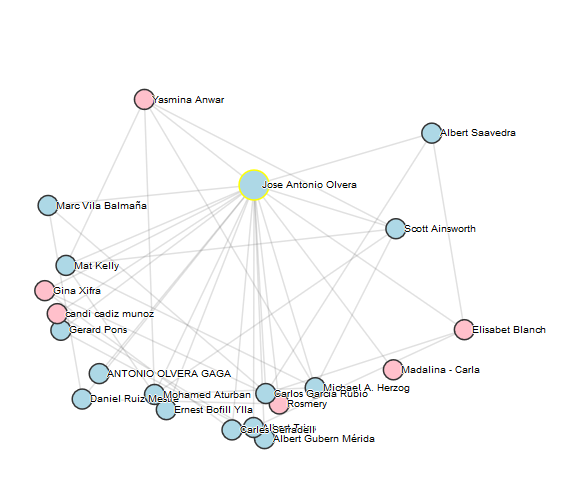
\includegraphics[scale=.85]{images/gender-graph.png}
\caption*{\scriptsize Figure \ref{fig:gender} visualize gender relationship among Jose Olvera Followers.}
\end{figure}

\subsubsection{2.3.3 Test for Gender Homophily}
\vspace{5mm}
To test our graph for gender homophily we implemented $<homophily.py>$. The result of running the program is shown below:\\

\begin{lstlisting}[style=nonumbers]
	Starting Time: Wed,  Mar 16, 2016 at 21:50:36
		
	Number of females: 6
	Number of males: 18
	p: 0.750
	q: 0.250
	2pq: 0.375
		
	Cross-gender edges:
	------------------
		
	Elisabet Blanch <--> David Plaza
	Yasmina Anwar <--> Michael A. Herzog
	Yasmina Anwar <--> Mohamed Aturban
	Yasmina Anwar <--> Mat Kelly
	Jose Antonio Olvera <--> Rosmery
	Daniel Ruiz Mestre <--> Rosmery
	Marc Vila Balmana <--> Rosmery
	Carlos Garcia Rubio <--> Gina Xifra
	Jose Antonio Olvera <--> Gina Xifra
	Carles Serradell <--> Gina Xifra
	Elisabet Blanch <--> Carlos Garcia Rubio
	Elisabet Blanch <--> Albert Trias
	candi cadiz munoz <--> Jose Antonio Olvera
	Yasmina Anwar <--> Jose Antonio Olvera
	Madalina - Carla <--> Jose Antonio Olvera
	Elisabet Blanch <--> Jose Antonio Olvera
	Yasmina Anwar <--> Scott Ainsworth
	Yasmina Anwar <--> Justin F Brunelle
	candi cadiz munoz <--> Albert Gubern Merida
	Albert Saavedra <--> Elisabet Blanch
		
	Summary of Cross-gender edges: 20 out of 52
	Percentage of Cross-gender edges 0.385
		
	End Time:  Wed,  Mar 16, 2016 at 21:50:36
	Execution Time: 0.00 seconds
\end{lstlisting}

\vspace{5mm}
As we can see 2pq $<$ cross-edges, 0.375 $<$ 0.385 $\therefore$ there is no evidence of homophily. 
\end{homeworkProblem}

%----------------------------------------------------------------------------------------
%	Bibliography
%----------------------------------------------------------------------------------------
\newpage
\begin{thebibliography}{9}
%\bibitem{Lutz} 
%Lutz, Mark (2013). List and Dictionaries. \textit{Learning Python} (5th ed.). (pp. %262-263). Sebastopol, CA: O'Reilly Media.
%
\bibitem{tweepy}
Tweepy API. (n.d.) Retrieved March 10, 2016, from \url{http://docs.tweepy.org/en/latest/api.html}

\bibitem{zooming}
Zooming and dragging. (n.d.) Retrieved March 10, 2016, from \url{http://bl.ocks.org/mbostock/6123708}

\bibitem{tip-tool}
d3-tip tool. (n.d.) Retrieved March 10, 2016, from \url{ http://bl.ocks.org/Caged/6476579}

\bibitem{directed}
Directed graph. (n.d.) Retrieved March 10, 2016, from \url{http://bl.ocks.org/mbostock/1153292}

\bibitem{polish-books}
Polish Books. (n.d.) Retrieved March 10, 2016, from \url{http://p.migdal.pl/wizualizacja-wolnych-lektur/polish_books_themes.html}

\bibitem{d3-markers}
D3 Markers. (n.d.) Retrieved March 10, 2016, from \url{http://bl.ocks.org/dustinlarimer/5888271}
\end{thebibliography}
\end{document}
